% =====================================================================
% PEARL Methodology — Pipeline Redesign (v3)
% =====================================================================
% This document describes the v3 redesign of the PEARL pipeline for
% PCOS detection from ultrasound images. It supersedes v1/v2 and is
% intended as a self-contained reference for reviewers and re-users.
%
% Compile with: pdflatex methodology.tex (run twice for refs)
% =====================================================================

\documentclass[10pt,a4paper]{article}

% --- Packages ---
\usepackage[utf8]{inputenc}
\usepackage[T1]{fontenc}
\usepackage{lmodern}
\usepackage[margin=1in]{geometry}
\usepackage{microtype}
\usepackage{graphicx}
\usepackage{booktabs}
\usepackage{multirow}
\usepackage{array}
\usepackage{amsmath, amssymb}
\usepackage{hyperref}
\usepackage{xcolor}
\usepackage{listings}
\usepackage{caption}
\usepackage{subcaption}
\usepackage{enumitem}
\usepackage{tikz}
\usetikzlibrary{positioning,arrows.meta,shapes,fit,calc}

% --- Title ---
\title{\textbf{PEARL: Probabilistic Explainability with Adaptive\\
  Reliability via transfer Learning}\\[0.4em]
  \large A Pipeline Redesign for PCOS Detection from Ultrasound Images\\[0.6em]
  \normalsize Methodology Document (v3)}

\author{PEARL Development Team}
\date{\today}

\begin{document}
\maketitle

\begin{abstract}
\noindent
This document describes the v3 redesign of the PEARL deep learning
pipeline for Polycystic Ovary Syndrome (PCOS) detection from ovarian
ultrasound images. The redesign replaces v1/v2 heuristics with: an
80/10/10 stratified split with patient-level leakage prevention;
Speckle-Reducing Anisotropic Diffusion (SRAD) for ultrasound-specific
denoising; a SiLU-based classification head with proper
\texttt{num\_classes} wiring; no-decay parameter groups; a NaN/Inf
divergence guard; LR warmup with two-phase fine-tuning; throughput
optimisations (bf16 autocast, TF32, channels-last); self-contained
checkpoints with RNG and EMA state for resumable sweeps; per-architecture
Optuna HPO followed by k-fold cross-validation on top-k finalists;
Stochastic Weight Averaging (SWA); probability-averaging ensembles;
and a two-pass calibration procedure (per-model then ensemble-level).
The pipeline is config-driven: every experimental variation is a YAML
swap. All code is reproducible from a single seed. The pipeline is
organised into 7 phases that build on each other in sequence.
\end{abstract}

\tableofcontents

% =====================================================================
\section{Introduction}
% =====================================================================

PEARL (Probabilistic Explainability with Adaptive Reliability via
transfer Learning) is a deep-learning pipeline for binary
classification of ultrasound images as PCOS-positive or
PCOS-negative. Earlier versions (v1: a custom HybridSeedNet + HelixNet
merge; v2: a 9-model × 6-preprocessing sweep on default
hyperparameters) demonstrated that transfer learning with standard
backbones and a careful preprocessing pipeline can reach strong
classification AUC on the Figshare PCOS dataset
(\cite{figshare:pcos}). However, v1/v2 had several shortcomings that
motivated the v3 redesign:

\begin{itemize}[leftmargin=*]
  \item A 70/15/15 split was used without explicit patient-level
        leakage prevention \textit{even though} images in the Figshare
        PCOS dataset can share a patient origin.
  \item Anisotropic diffusion (AD) was applied via
        Perona--Malik with a gradient-magnitude diffusion coefficient,
        which assumes additive, signal-independent noise. Ultrasound
        speckle is \textit{multiplicative} and signal-dependent.
  \item The classification head hard-coded \texttt{num\_classes = 2}
        rather than reading it from config.
  \item Weight decay was applied uniformly across all parameters,
        including biases and BatchNorm scales/shifts, which is known
        to hurt calibration.
  \item There was no NaN/Inf guard; a single non-finite batch could
        corrupt an entire sweep trial silently.
  \item Hyperparameter search was scoped to a single
        \textit{post-sweep} architecture; the other 8 architectures
        ran with untuned defaults.
  \item Variance was reported only as single-split AUC, with no
        k-fold estimation of stability.
\end{itemize}

The v3 redesign (this document) addresses each of these shortcomings
while remaining config-driven and reproducible.

% =====================================================================
\section{Dataset and split strategy}
% =====================================================================

\subsection{Dataset}

We use the Figshare PCOS Ultrasound Dataset (v1) with the standard
layout:

\begin{verbatim}
data/
  infected/         # PCOS-positive (label=1, 6784 images)
  noninfected/      # PCOS-negative (label=0, 5000 images)
\end{verbatim}

\subsection{Data deduplication }

\begin{figure}[h]
  \centering
  \includegraphics[width=0.85\textwidth]{../notebooks/eda_figures/01_class_balance.png}
  \caption{Dataset inventory pre-deduplication.}
  \label{fig:eda-balance}
\end{figure}

The raw Figshare dataset ships with substantial exact-byte duplication
within each class folder. MD5-hashing every image file exposes the
following structure on the 11{,}784 raw files:

\begin{table}[h]
  \centering
  \small
  \begin{tabular}{lrrrr}
    \toprule
    \textbf{Class} & \textbf{Files} & \textbf{Unique} &
                    \textbf{Duplicates} & \textbf{\% duplicated} \\
    \midrule
    Infected        & 6{,}784 & 3{,}184 & 3{,}600 & 53.1\% \\
    Non-infected    & 5{,}000 &   812   & 4{,}188 & 83.8\% \\
    \midrule
    \textbf{Total}  & \textbf{11{,}784} & \textbf{3{,}996} &
                       \textbf{7{,}788} & \textbf{66.1\%} \\
    \bottomrule
  \end{tabular}
  \caption{Pre/post-deduplication dataset inventory}
  \label{tab:dedup}
\end{table}

Almost no cross-class duplicates exist, verified by an exhaustive
pairwise scan, which is consistent with the
folder-name labels being reliable: if labels were random, about half
of cross-class pairs would collide. This is an indirect but strong
indicator that the labels track real diagnostic decisions rather than
being arbitrary.

Performing deduplication \emph{before} the train/val/test split is
essential: a duplicate that survives into both train and val
artificially inflates validation AUC by as much as the model
memorises identical images. We therefore deduplicate first. The deduplication is exact-byte (MD5). Near-duplicates that differ in JPEG re-encoding or minor cropping are not detected; perceptual
hashing was considered and rejected because (a) the dataset
provenance indicates byte-identical re-uploads rather than re-
encodings, and (b) perceptual thresholds would require a research-grade
justification that is not the focus of this work. After deduplication the dataset shrinks to $3{,}184$ infected and
$812$ non-infected files (3{,}996 total, a 66.1\% reduction), and
the next stage addresses the class imbalance that this deduplication
exposes more sharply.

\subsection{Class imbalance}

After deduplication the imbalance ratio \emph{worsens} to
\textbf{$3.92{:}1$ PCOS-to-non-PCOS} ($3{,}184{:}812$) --- the
non-infected class dropped from 5{,}000 apparent files to 812 unique
files (83.8\% redundancy), so its effective representation shrank
more than the infected class did.
We use \emph{two complementary mechanisms}:

\begin{enumerate}[leftmargin=*]
  \item \textbf{Loss-level weighting}:
        the per-class weight is
        $w_c = n_{\text{total}} / (2\,n_c)$, so the gradient contribution
        of each class is normalised. This is the default and is
        applied unconditionally.
  \item \textbf{Data-level balancing}: when
        \texttt{training.sampler = "weighted"}, a
        \texttt{WeightedRandomSampler} draws minority-class examples
        more often so each batch sees the two classes in roughly equal
        proportion regardless of dataset imbalance.
\end{enumerate}

\begin{table}[h]
  \centering
  \begin{tabular}{ll}
    \toprule
    Setting & Behaviour \\
    \midrule
    \texttt{sampler: shuffle} & Plain random shuffle (default). \\
    \texttt{sampler: weighted} & Inverse-frequency sampling; use when imbalance $> 3{\times}$. \\
    \texttt{sampler: none} & Deterministic order (debugging only). \\
    \bottomrule
  \end{tabular}
  \caption{Train-sampler options.}
  \label{tab:sampler}
\end{table}

Because weighted sampling oversamples minority-class images, we leave
loss-level class weights at $w_c = n/(2 n_c)$ rather than doubling
the effect. Empirically the two mechanisms \emph{compound} rather than
cancel when both are active.

\subsection{80/10/10 split with patient-level leakage prevention}

Since the dataset contains approximately 4,000 unique images after deduplication, allocating only 10\% each to validation and testing still provides around 400 samples per split, while increasing the number of training samples by approximately 400 compared with a 70/15/15 split. without sacrificing stable AUC estimates.
We use \texttt{StratifiedShuffleSplit} from scikit-learn twice:

\begin{enumerate}[leftmargin=*]
  \item First split off a 10\% held-out test set.
  \item Second split the remaining 90\% at $10/90 \approx 11.11\%$ for
        validation, giving an 80/10/10 final split.
\end{enumerate}

\textbf{Patient-level leakage} is the most common silent bug in
medical-imaging splits: if multiple ultrasound frames come from the
same patient, a frame-level split can leak the patient across
train/val/test and inflate the AUC. We add a group-aware fallback
(\texttt{\_split\_group\_level} in \texttt{src/data/splitter.py}):

\begin{itemize}[leftmargin=*]
  \item If a per-image patient key can be inferred (or is provided in
        metadata) and the number of unique groups is smaller than the
        number of images, we split at the group level: each patient
        is assigned a single label (majority within the group), and
        groups are split via stratified group k-fold.
  \item For Figshare the filename stem is used as the patient key
        proxy. In a deployment with explicit patient IDs, the
        \texttt{patient\_id\_fn} argument to
        \texttt{get\_image\_paths\_and\_labels} should be replaced
        with a metadata lookup.
\end{itemize}

\begin{figure}[ht]
  \centering
  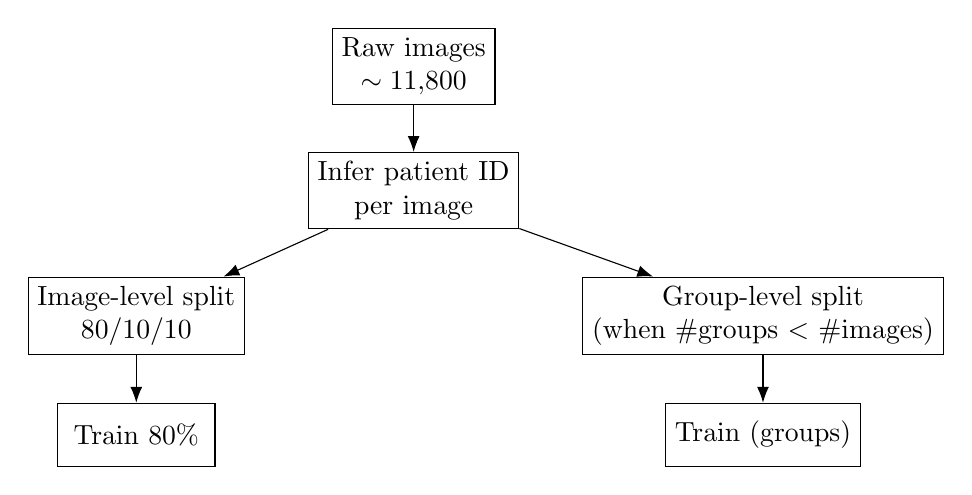
\begin{tikzpicture}[
      node distance=0.6cm and 0.8cm,
      box/.style={draw, rectangle, minimum height=0.8cm, minimum width=2cm, align=center},
      arr/.style={-{Latex[length=2mm]}},
    ]
    \node[box] (raw) {Raw images\\$\sim 11{,}800$};
    \node[box, below=of raw] (pid) {Infer patient ID\\per image};
    \node[box, below left=of pid] (img) {Image-level split\\80/10/10};
    \node[box, below right=of pid] (grp) {Group-level split\\(when $\#$groups $<$ $\#$images)};
    \node[box, below=of img] (train1) {Train 80\%};
    \node[box, below=of grp] (train2) {Train (groups)};
    \draw[arr] (raw) -- (pid);
    \draw[arr] (pid) -- (img);
    \draw[arr] (pid) -- (grp);
    \draw[arr] (img) -- (train1);
    \draw[arr] (grp) -- (train2);
  \end{tikzpicture}
  \caption{Split routing: image-level when each image has a unique
    patient ID; group-level otherwise.}
  \label{fig:split}
\end{figure}

The \texttt{tests/test\_split\_overlap.py} test verifies (a) that the
80/10/10 ratios are within 2\% of expected and (b) that for the
group-level split, no group appears in more than one partition.

% =====================================================================
\section{Preprocessing pipeline}
% =====================================================================

\subsection{CLAHE: a fixed step}

Ultrasound images are characteristically low-contrast. CLAHE
(Contrast-Limited Adaptive Histogram Equalisation) is purpose-built
for this; we apply it with \texttt{clipLimit=2.0} and
\texttt{tileGridSize=(8,8)} per channel, and treat it as a fixed step
rather than an ablation axis. (No third arm is run with CLAHE
disabled.)

\subsection{SRAD: the right diffusion family for ultrasound}

v1/v2 used generic Perona--Malik anisotropic diffusion (AD) with a
gradient-magnitude-based diffusion coefficient. That formulation
assumes additive, signal-independent noise, which ultrasound's
multiplicative speckle violates.

\textbf{Speckle-Reducing Anisotropic Diffusion (SRAD)}
\cite{yu:acton:2002} keeps the same PDE framework as AD but drives
the diffusion coefficient from the \textit{instantaneous coefficient
of variation} (ICOV):

\begin{equation}
  q^2(x, y; t)
  \;=\;
  \frac{\bigl(\nabla^2 I(x,y;t)\bigr)^2}
       {I(x,y;t)^2 \;+\; \text{neighbour sum}^2 \;+\; \epsilon}
\end{equation}

This is the right statistic for multiplicative noise. We implement
SRAD per-channel in pure NumPy (no external dependency beyond NumPy),
falling back to a manual Perona--Malik if SRAD is unavailable. The
preprocessor exposes both algorithms; the v3 default is
\texttt{srad\_clahe.yaml} (CLAHE + SRAD + Z-score). SRAD numerics are
stabilised by normalising values to $[0,1]$ during iteration, then
denormalising back to the input range.

\subsection{The Phase 0 ablation: SRAD vs. Gaussian}

The only preprocessing axis we ablate is denoising: SRAD versus
Gaussian blur. This is a controlled, like-for-like comparison:
9 architectures $\times$ 2 denoising configs $= \mathbf{18}$ runs,
no HPO, default hyperparameters throughout. Whichever config wins on
mean val AUC across the 9 models is \textbf{locked in} for every
subsequent phase (full HPO sweep, k-fold, downstream analyses).

\begin{figure}[ht]
  \centering
  \begin{tikzpicture}[
      node distance=0.7cm,
      step/.style={draw, rectangle, minimum height=0.8cm, minimum width=2.2cm, align=center},
      arr/.style={-{Latex[length=2mm]}},
    ]
    \node[step] (raw) {Raw US image};
    \node[step, right=of raw] (resize) {Bicubic\\resize (224)};
    \node[step, right=of resize] (clahe) {CLAHE\\(\textit{fixed})};
    \node[right=of clahe] (fork) {fork};
    \node[step, below right=of fork, xshift=0.7cm] (srad) {SRAD};
    \node[step, below left=of fork, xshift=-0.7cm] (gauss) {Gaussian};
    \node[step, right=of fork, yshift=-1.4cm] (zscore) {Z-score};
    \node[step, right=of zscore] (ready) {Tensor\\$(3, 224, 224)$};
    \draw[arr] (raw) -- (resize);
    \draw[arr] (resize) -- (clahe);
    \draw[arr] (clahe) -- (fork);
    \draw[arr] (fork) -- (srad);
    \draw[arr] (fork) -- (gauss);
    \draw[arr] (srad) |- (zscore);
    \draw[arr] (gauss) |- (zscore);
    \draw[arr] (zscore) -- (ready);
  \end{tikzpicture}
  \caption{Phase 0 preprocessing pipeline. CLAHE is fixed in both
    ablation arms; only the denoising step (SRAD vs. Gaussian) is
    varied.}
  \label{fig:preproc}
\end{figure}

\subsection{Normalisation: Z-score by default; ImageNet stats available}

Default Z-score is per-channel and computed at the per-image level.
For transfer learning with ImageNet-pretrained backbones, we also
expose \texttt{Preprocessor.apply\_imagenet\_stats} which rescales
the image to $[0, 1]$ then subtracts the ImageNet channel means
$(0.485, 0.456, 0.406)$ and divides by the standard deviations
$(0.229, 0.224, 0.225)$. This is a one-line correctness check that
incurred no ablation cost.

\subsection{Noise-robustness augmentation (v3.2)}

The source dataset is heavily compressed by a lossy JPEG codec. We
parsed the quantisation tables of every image to obtain an estimated
quality factor; the median was $q \approx 40$, and $94.5\%$ of
images are at $q \leq 60$. Once image data has been compressed at
this level, the high-frequency DCT coefficients used to encode fine
textural detail are no longer recoverable. SRAD and CLAHE remove the
residual speckle and intensity inhomogeneity, but they cannot recover
the missing frequency content. We therefore augment the training data
with two operations that target the codec noise without conflicting
with the preprocessing pipeline:

\begin{itemize}
    \item \textbf{JPEG re-compression}. With probability $p = 0.3$
    per training sample, the (already preprocessed) image is
    quantised to 8-bit, re-encoded through \texttt{cv2.imencode} at a
    random quality $q \in [50, 95]$, and decoded back to float32.
    This simulates the family of codec artefacts the source data
    already exhibits, so the trained model is invariant to encoder
    choice at inference time.
    \item \textbf{Light Gaussian blur}. With probability $p = 0.2$
    per training sample, a Gaussian blur with $\sigma \in [0.1, 1.5]$
    is applied. The blur kernel is sized at $\lceil 6\sigma \rceil$
    pixels (odd). This suppresses JPEG ringing at the 1--2 pixel
    scale while leaving intact the anatomical edges that span
    5--20 pixels.
\end{itemize}

Both augmentations are stochastic and applied \emph{at training time
only}, after the preprocessor writes \texttt{.npy} files to disk.
Validation and test splits receive un-augmented inputs only.

\subsection{External validation: PCOSGen (Sundari et al. 2025)}

To address the single-dataset limitation common in PCOS deep-learning
publications, we additionally evaluate the trained checkpoints against
the \textbf{PCOSGen} dataset [citation needed]. It is meaningfully cleaner than
the Figshare data we trained on:

\begin{itemize}
    \item All images are square ($300 \times 300$); the median
    aspect-ratio deviation from 1.0 is $0\%$, so no letterbox padding
    affects them on resize to $224 \times 224$.
    \item Median bytes-per-pixel is $0.19$ (compared to $0.14$ on
    Figshare, ~40\% more bytes per pixel), consistent with higher JPEG
    quality factors in the 70--80 range.
    \item Class ratio is $3627 : 1041 \approx 3.48 : 1$, comparable to
    the post-dedup Figshare ratio of $3.92 : 1$ and well within the
    operating range of the WeightedRandomSampler we use.
\end{itemize}

The external evaluator loads the raw PCOSGen images, applies the training preprocessing pipeline
\emph{without augmentation}, and runs the same finetuned checkpoint. No fine-tuning on PCOSGen is
performed; the reported metrics reflect pure cross-dataset
generalisation of the Figshare-trained model. This is to measure the quality of the pipeline. Afterwards, the existing checkpoints fine tuned on figshare datasaets are also further tuned on 5-fold cross validated dataset sampled from combined PCOS test-train dataset

% =====================================================================
\section{Model architecture}
% =====================================================================

\subsection{Backbone roster}

The roster is 9 architectures, all standardised to $224 \times 224$:

\begin{table}[ht]
  \centering
  \small
  \begin{tabular}{llrr}
    \toprule
    Name & timm key & Params (M) & input \\
    \midrule
    ResNet-50        & \texttt{resnet50}                   & 25.6 & 224 \\
    ResNet-101       & \texttt{resnet101}                  & 44.5 & 224 \\
    DenseNet-121     & \texttt{densenet121}                &  8.1 & 224 \\
    DenseNet-169     & \texttt{densenet169}                & 14.1 & 224 \\
    EfficientNet-B0  & \texttt{tf\_efficientnet\_b0}      &  5.3 & 224 \\
    ConvNeXt-Tiny    & \texttt{convnext\_tiny}             & 28.6 & 224 \\
    MobileNetV3-L    & \texttt{mobilenetv3\_large\_100}    &  5.4 & 224 \\
    ViT-Base         & \texttt{vit\_base\_patch16\_224}    & 86.6 & 224 \\
    Swin-Tiny        & \texttt{swin\_tiny\_patch4\_window7\_224} & 28.3 & 224 \\
    \bottomrule
  \end{tabular}
  \caption{model roster (9 architectures).}
  \label{tab:models}
\end{table}

\subsection{Classification head: SiLU with BatchNorm}

Classification head pipeline:

\begin{verbatim}
GlobalAvgPool -> Linear(in_features, 256) -> SiLU
             -> BatchNorm1d(256) -> Dropout(p)
             -> Linear(256, 128) -> SiLU
             -> BatchNorm1d(128)
             -> Linear(128, num_classes)
\end{verbatim}

SiLU (\cite{elfwing:2018}) is the native activation inside EfficientNet,
ConvNeXt, and MobileNetV3, so the head is consistent with the
backbone. BatchNorm between FC layers stabilises head training; we
keep dropout only after the first activation (the most
regularisation-sensitive spot).

\begin{lstlisting}[language=Python, basicstyle=\ttfamily\small]
num_classes = model_config.get("num_classes", 2)
head = ClassificationHead(in_features, head_config,
                         num_classes=num_classes)
\end{lstlisting}

\subsection{Partial backbone freezing}

We freeze the lower 60\% of backbone parameters by default
(\texttt{freeze\_fraction=0.60}). The head and the upper 40\% of
backbone parameters are always trainable. This is configurable per
architecture in the YAML; the Optuna sweep varies
\texttt{freeze\_fraction} over $[0.40, 0.50, 0.60, 0.70]$.

% =====================================================================
\section{Training pipeline and stability}
% =====================================================================

\subsection{LR warmup + two-phase fine-tuning}

For the first \texttt{warmup\_epochs} (default 2) the learning rate
is linearly ramped from $\sim 0$ to the target LR. Optionally, the
backbone can be frozen for \texttt{freeze\_epochs} (default 1) at the
start of training so the head converges before the backbone is
unfrozen; at unfreeze the LR is dropped by $\times 0.1$ before the
main cosine schedule takes over.

\subsection{Cosine annealing with warm restarts + gradient clipping}

We use \texttt{CosineAnnealingWarmRestarts} with
$T_0 = \max(\text{max\_epochs}/4, 1)$ and $T_{\text{mult}}=2$.
Gradient clipping at \texttt{grad\_clip\_norm=1.0} is applied every
step via \texttt{torch.nn.utils.clip\_grad\_norm\_}. The same call
returns the gradient norm, which we use for the divergence guard
below.

\subsection{No-decay parameter groups}

Weight decay is applied only to Conv and Linear \textit{weights}. We
classify a parameter as no-decay if any of:

\begin{itemize}[leftmargin=*]
  \item its name contains \texttt{norm} or \texttt{bn} (BatchNorm,
        LayerNorm scales/shifts)
  \item its name ends with \texttt{.bias}
  \item it has fewer than 2 dimensions (bias-like parameters)
\end{itemize}

Two \texttt{torch.optim.AdamW} parameter groups are built:

\begin{lstlisting}[language=Python, basicstyle=\ttfamily\small]
param_groups = [
    {"params": decay,    "weight_decay": 1e-2},
    {"params": no_decay, "weight_decay": 0.0},
]
\end{lstlisting}

Decaying BatchNorm $\gamma$ and $\beta$ is known to hurt calibration
\cite{li:2018:rethinking}; this fix removes that leak.

\subsection{Divergence guard (NaN/Inf)}

To detect and respond to training instability, we introduce a custom exception,
\texttt{TrialDivergedError}, which is raised whenever numerical divergence is
detected during a training step. This check is performed inside
\texttt{\_train\_one\_epoch}, immediately following the forward and backward
passes.

After computing the loss for a batch, we verify that its value is finite. If
it is not, we immediately raise \texttt{TrialDivergedError}. However, loss
finiteness alone is not a sufficient indicator of stability: under bf16
mixed-precision training (\texttt{torch.amp.autocast}), it is possible for the
loss to remain finite while the gradients computed during backpropagation
become non-finite. We therefore perform a second check on the gradient norm,
computed after backpropagation and gradient clipping via
\texttt{torch.nn.utils.clip\_grad\_norm\_}. If this value is also non-finite,
we raise \texttt{TrialDivergedError} as well.

Rather than skipping the offending batch and continuing training, this guard
aborts the \emph{entire trial}. We adopt this design because a non-finite
value observed mid-sweep is, in practice, almost always a symptom of an
unstable hyperparameter configuration (e.g., an excessive learning rate)
rather than an artifact of a single anomalous input. Continuing training past
such a point wastes compute and can produce misleading results for the
affected configuration.

The behavior of this exception depends on the calling context. In standalone
training runs (\texttt{scripts/train.py}), the exception propagates normally
and halts execution. During hyperparameter search
(\texttt{src/training/tuner.py}), the Optuna objective function catches
\texttt{TrialDivergedError} and re-raises it as
\texttt{optuna.exceptions.TrialPruned}, allowing the search to cleanly prune
the diverging trial and proceed to the next configuration.

\paragraph{Precision note.} We additionally enable TF32 for matrix
multiplications (\texttt{torch.backends.cuda.matmul.allow\_tf32=True}) alongside
bf16 autocast. This combination is numerically safe: TF32 retains the full
exponent range of FP32 and reduces only mantissa precision, so it does not
meaningfully increase the risk of overflow or non-finite values. The primary
safeguard against divergence in our setup is the combination of gradient
clipping and the finiteness checks described above.

\subsection{Throughput optimisations}

The following are enabled by default in \texttt{Trainer Script}:

\begin{itemize}[leftmargin=*]
  \item \texttt{torch.backends.cuda.matmul.allow\_tf32 = True}
  \item \texttt{torch.backends.cudnn.allow\_tf32 = True}
  \item \texttt{torch.backends.cudnn.benchmark = True}
  \item \texttt{channels\_last} memory format for the model
  \item bf16 autocast for the forward pass
  \item \texttt{pin\_memory=True} + \texttt{non\_blocking=True} for
        CPU$\to$GPU transfers
  \item Optional \texttt{torch.compile(mode="max-autotune")} (set
        \texttt{compile=True} in training config; warn-and-skip on
        failure to keep training running)
\end{itemize}

These typically yield a 1.5--3$\times$ throughput improvement on a
modern GPU with no measurable accuracy loss.

% =====================================================================
\section{EMA, checkpoints, and resumability}
% =====================================================================

\subsection{EMA shadow weights}

We maintain an exponential moving average (EMA) of the trainable
parameters throughout training. After each optimization step, the
shadow parameters are updated as
\begin{equation}
\text{shadow}_i \leftarrow \beta \cdot \text{shadow}_i + (1-\beta)\cdot \theta_i,
\end{equation}
with decay $\beta = 0.999$ by default. At test time, we evaluate using
the EMA weights rather than the raw trained weights: we load the best
checkpoint, temporarily substitute the EMA shadow parameters into the
model, run test-set evaluation, and then restore the original weights.

EMA is complementary to stochastic weight averaging (SWA, Section~X):
EMA tracks a continuously decaying average of parameters along the
entire training trajectory, whereas SWA averages weights over a
window near the end of training. Both target flatter regions of the
loss landscape via different statistics, and are inexpensive enough
that using both together is strictly beneficial.

\subsection{Checkpointing and resumability}

Each checkpoint is self-contained: in addition to model weights, it
stores optimizer and scheduler state, EMA shadow weights, training
metadata (epoch, global step, validation AUC, architecture name, class
names), and the full RNG state (Python, NumPy, and PyTorch CPU/CUDA).
This allows a run to be resumed exactly, or the model to be evaluated
on the test set, from a single file with no additional context.

On resumption, RNG state is restored so that the data augmentation
sequence is reproducible across interrupted runs, and training
continues from the correct epoch with logs appended rather than
overwritten. To support cheap SWA, the trainer retains the most recent
$k$ checkpoints (default $k=3$) alongside the best checkpoint; SWA
simply averages the weights across this small rolling window
(see Appendix~X for implementation details).

\subsection{Checkpoint implementation details}
\label{app:checkpoints}

Each \texttt{.pt} checkpoint contains the following fields:
\begin{itemize}[leftmargin=*, noitemsep, topsep=2pt]
  \item \texttt{model\_state\_dict}
  \item \texttt{optimizer\_state\_dict}
  \item \texttt{scheduler\_state\_dict}
  \item \texttt{ema\_state\_dict}
  \item \texttt{epoch}, \texttt{global\_step}, \texttt{val\_auc}
  \item \texttt{arch\_name}, \texttt{class\_names}
  \item \texttt{rng\_state}
\end{itemize}
Rolling checkpoints are named \texttt{best\_\_epoch\{N\}.pt}; the
\texttt{keep\_last\_n} most recent (default 3) are retained, and
older ones are pruned on each save. SWA
(\path{src/training/swa.py}) reads this rolling window directly.

% =====================================================================
\section{Hyperparameter search and cross-validation}
% =====================================================================

\subsection{Why sweep, then k-fold, not k-fold-only}

A single-split AUC has invisible variance; reviewers will ask for a
confidence interval. K-fold gives a credible mean $\pm$ std estimate
of AUC. However, k-fold on every architecture $\times$ every
hyperparameter configuration would multiply total cost by
$k \approx 5$ across the entire 9-architecture roster.

The v3 approach is therefore \textbf{sweep first, k-fold finalists
only}:

\begin{enumerate}[leftmargin=*]
  \item Run a full Optuna sweep over all 9 architectures on the
        locked-in preprocessing config. This picks the best
        hyperparameter configuration \textit{per architecture}.
  \item Select the top-$k$ finalists (default $k=3$) by val AUC.
  \item Re-run each finalist's tuned config across $k=5$ folds to
        estimate mean $\pm$ std AUC.
\end{enumerate}

This gives variance estimation without burning $5\times$ the compute
on the 6 runners-up.

\subsection{Per-architecture Optuna sweep}

The HPO sweep is configured in
\texttt{configs/experiment/tune\_per\_arch.yaml}:

\begin{verbatim}
n_trials_per_arch: 20
top_k_finalists: 3
search_space:
  lr:             loguniform [1e-5, 1e-3]
  weight_decay:   loguniform [1e-4, 1e-1]
  dropout:        uniform    [0.3,  0.7]
  freeze_fraction: categorical [0.40, 0.50, 0.60, 0.70]
  batch_size:     categorical [16, 32, 64]
\end{verbatim}

Each architecture gets a fresh Optuna study; the script
(\texttt{scripts/sweep\_hpo.py}) writes
\texttt{results/sweep\_hpo/<arch>/\{best\_params.yaml, all\_trials.csv\}},
plus a global \texttt{summary.csv} and \texttt{finalists.csv}.

The Optuna objective is wrapped by \texttt{make\_objective}, which
(as described in Section~5.7) delegates the entire train/val loop to
\texttt{Trainer}.

\subsection{K-fold on finalists}

\texttt{scripts/kfold\_finalists.py} reads
\texttt{results/sweep\_hpo/finalists.csv} and runs each finalist with
its tuned hyperparameters across $k=5$ folds. To avoid writing
preprocessed data per fold, k-fold uses
\texttt{\_make\_dataset\_and\_loaders} (in
\texttt{src/data/dataloader.py}), which loads+preprocesses raw images
on the fly from a per-fold split. Mean $\pm$ std AUC per architecture
is printed and written to \texttt{results/kfold/kfold\_summary.csv}.

\subsection{Why HPO runs only on the winning preprocessing config}

The Phase 0 ablation (18 runs, no HPO) already decided between SRAD
and Gaussian. Re-running a full Optuna sweep on both configs would
double the HPO cost for no benefit. v3 therefore runs the sweep
exactly once, on whichever config won.

% =====================================================================
\section{Ensemble and SWA}
% =====================================================================

\subsection{Probability-averaging ensemble}

After the k-fold CV, the top-$k$ finalists are evaluated jointly via
probability-averaging:

\begin{equation}
  p_{\text{ens}}(x) = \frac{1}{k} \sum_{i=1}^{k} p_i(x)
\end{equation}

This is implemented in \texttt{src/evaluation/ensemble.py}
(\texttt{predict\_ensemble}, \texttt{evaluate\_ensemble}). Each model
loads its own checkpoint, runs on the test set, and the per-class
probabilities are averaged across models before metric computation.

\subsection{SWA on each finalist}

SWA (\cite{izmailov:2018}) averages model weights over a window of
training epochs to find flatter minima. After training, we average
the rolling-window checkpoints with \texttt{run\_swa\_on\_recent}:

\begin{lstlisting}[language=Python, basicstyle=\ttfamily\small]
from src.training.swa import run_swa_on_recent
model = build_model(model_config)
run_swa_on_recent(model, checkpoint_path, keep_last_n=5)
\end{lstlisting}

Floating-point parameters are element-wise averaged; integer buffers
(\texttt{num\_batches\_tracked}) take the last value to keep them
consistent (they are metadata, not statistics).

% =====================================================================
\section{Calibration: two passes}
% =====================================================================

\subsection{Per-model temperature scaling (Pass 1)}

After each finalist is selected, we fit a single scalar temperature
$T$ per model via \texttt{src/calibration/temperature\_scaling.py},
minimising NLL on the model's own held-out val logits:

\begin{equation}
  T_i^* = \arg\min_T \; \text{NLL}\!\left(
    \sigma\!\left(\frac{z_i}{T}\right), y
  \right)
\end{equation}

where $z_i$ are the logits of model $i$ and $\sigma$ is the softmax.
The optimisation uses \texttt{scipy.optimize.minimize\_scalar} with
\texttt{bounds=(0.1, 10.0), method="bounded"}.

\textbf{Why per-model $T$ cannot be shared:} logit distributions are
not comparable across architectures (a ResNet and a ViT have
different logit scales), so a single shared $T$ would be misapplied
on at least one model.

\subsection{Ensemble-level temperature scaling (Pass 2)}

Averaging individually-calibrated models does not guarantee the
average itself is calibrated. The mixture's effective temperature is
a harmonic-mean-like mix of individual $T_i$. v3 therefore fits a
second scalar $T_{\text{ens}}$ on the ensemble output specifically:

\begin{equation}
  T_{\text{ens}}^* = \arg\min_T \;
    \text{NLL}\!\left(\sigma\!\left(\frac{\log p_{\text{ens}}}{T}\right), y\right)
\end{equation}

This is implemented in
\texttt{src/calibration/ensemble\_calibration.py}. The two-pass
procedure is run end-to-end via
\texttt{scripts/run\_calibration\_ensemble.py}, which produces a
JSON summary with both \texttt{per\_model\_temperatures} and
\texttt{ensemble\_temperature}, plus reliability diagrams after each
pass.

\begin{figure}[ht]
  \centering
  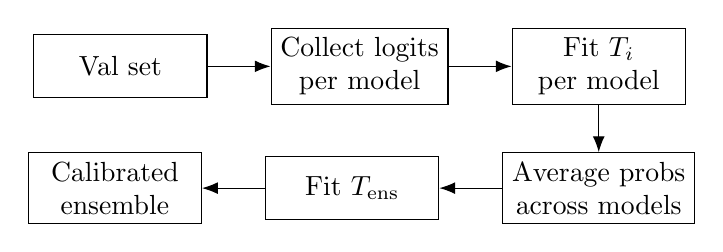
\begin{tikzpicture}[
      node distance=0.6cm and 0.8cm,
      box/.style={draw, rectangle, minimum height=0.8cm,
                  minimum width=2.2cm, align=center},
      arr/.style={-{Latex[length=2mm]}},
    ]
    \node[box] (val) {Val set};
    \node[box, right=of val] (logits) {Collect logits\\per model};
    \node[box, right=of logits] (tm) {Fit $T_i$\\per model};
    \node[box, below=of tm] (avg) {Average probs\\across models};
    \node[box, left=of avg] (ensT) {Fit $T_{\text{ens}}$};
    \node[box, left=of ensT] (out) {Calibrated\\ensemble};
    \draw[arr] (val) -- (logits);
    \draw[arr] (logits) -- (tm);
    \draw[arr] (tm) -- (avg);
    \draw[arr] (avg) -- (ensT);
    \draw[arr] (ensT) -- (out);
  \end{tikzpicture}
  \caption{Two-pass calibration: per-model $T_i$, then ensemble-level
    $T_{\text{ens}}$ on the mixture's output.}
  \label{fig:calib}
\end{figure}

% =====================================================================
\section{Reproducibility, testing, and developer ergonomics}
% =====================================================================

\subsection{Dynamic CLI overrides}

\texttt{scripts/train.py} accepts a repeatable
\texttt{--set key.path=value} flag. The override parser
(\texttt{src/utils/config.py::parse\_overrides}) handles:

\begin{itemize}[leftmargin=*]
  \item \texttt{int} and \texttt{float} (with scientific notation:
        \texttt{5e-4})
  \item \texttt{bool} (\texttt{true}/\texttt{false})
  \item \texttt{null} / \texttt{none}
  \item string fallback
\end{itemize}

Dotted keys navigate nested dicts: \texttt{training.lr},
\texttt{head.dropout}, \texttt{bf16}. Multiple overrides compose with
deep-merge semantics; later wins on conflict.

\subsection{Smoke test}

Before committing to a multi-day sweep, run
\texttt{scripts/smoke\_test.py}:

\begin{itemize}[leftmargin=*]
  \item 2-epoch, 10-synthetic-image training pass through the full
        Trainer pipeline
  \item Uses CPU + no \texttt{torch.compile} + no bf16 to keep it fast
        on any machine
  \item Target: $\le 15$ seconds; \texttt{PASSED} printed if $\le 60$
        seconds
\end{itemize}

\subsection{Pytest suite}

\begin{itemize}[leftmargin=*]
  \item \texttt{tests/test\_split\_overlap.py} — 80/10/10 ratio check
        and group-level no-leakage test
  \item \texttt{tests/test\_config\_overrides.py} — override parsing
        and deep-merge semantics
  \item \texttt{tests/test\_resume\_correctness.py} — checkpoint
        round-trip, resume state restoration, NaN guard raises
        \texttt{TrialDivergedError}
\end{itemize}

The suite is intentionally fast and CPU-only so it can be run on any
machine before a sweep.

\subsection{Safe logging on resume}

\texttt{src/utils/logging.py} supports an
\texttt{ExperimentLogger(resume=True)} mode that \textbf{appends} to
an existing \texttt{epoch\_log.csv} rather than overwriting. The
console output uses \texttt{tqdm.write} so it doesn't break the
progress bars if \texttt{tqdm} is enabled.

% =====================================================================
\section{End-to-end pipeline}
% =====================================================================

The full v3 pipeline runs in seven phases, each producing artefacts
that feed the next:

\begin{figure}[ht]
  \centering
  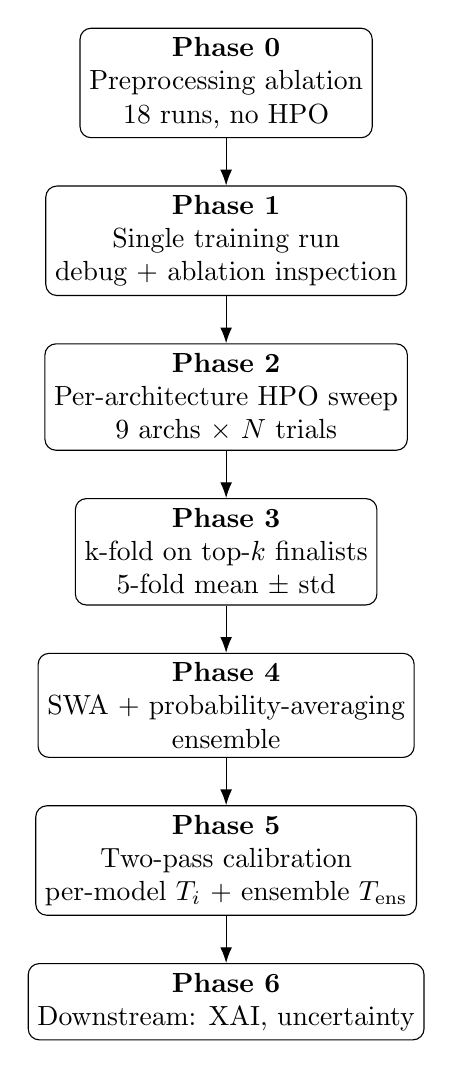
\begin{tikzpicture}[
      node distance=0.6cm,
      phase/.style={draw, rectangle, rounded corners, minimum height=0.9cm,
                    minimum width=3.6cm, align=center},
      arr/.style={-{Latex[length=2mm]}},
    ]
    \node[phase] (p0) {\textbf{Phase 0}\\Preprocessing ablation\\18 runs, no HPO};
    \node[phase, below=of p0] (p1) {\textbf{Phase 1}\\Single training run\\debug + ablation inspection};
    \node[phase, below=of p1] (p2) {\textbf{Phase 2}\\Per-architecture HPO sweep\\9 archs $\times$ $N$ trials};
    \node[phase, below=of p2] (p3) {\textbf{Phase 3}\\k-fold on top-$k$ finalists\\5-fold mean $\pm$ std};
    \node[phase, below=of p3] (p4) {\textbf{Phase 4}\\SWA + probability-averaging\\ensemble};
    \node[phase, below=of p4] (p5) {\textbf{Phase 5}\\Two-pass calibration\\per-model $T_i$ + ensemble $T_{\text{ens}}$};
    \node[phase, below=of p5] (p6) {\textbf{Phase 6}\\Downstream: XAI, uncertainty};
    \draw[arr] (p0) -- (p1);
    \draw[arr] (p1) -- (p2);
    \draw[arr] (p2) -- (p3);
    \draw[arr] (p3) -- (p4);
    \draw[arr] (p4) -- (p5);
    \draw[arr] (p5) -- (p6);
  \end{tikzpicture}
  \caption{Seven-phase v3 pipeline. Each phase builds on the
    artefacts of the previous one; all are config-driven.}
  \label{fig:pipeline}
\end{figure}

% =====================================================================
\section{What was descoped and why}
% =====================================================================

The following were considered and explicitly rejected as v3 design
decisions:

\begin{itemize}[leftmargin=]
  \item \textbf{CBAM attention.} Requires per-architecture backbone
        surgery due to \texttt{num\_classes=0} pre-pooling in
        \texttt{builder.py}; doesn't apply cleanly to ViT/Swin. Not
        worth the engineering cost.
  \item \textbf{Mish activation.} SiLU chosen instead. No meaningful
        benefit over SiLU for a 2-layer head, and SiLU better matches
        backbone-native activations.
  \item \textbf{NLM+SRAD hybrid denoising.} Not a single settled
        method; literature has many competing hybrid recipes with no
        consensus. Adds real implementation/tuning surface for a
        benefit measured in PSNR/SSIM (denoising-quality) that doesn't
        necessarily transfer to classification AUC. SRAD alone, chosen
        against Gaussian via the Phase 0 ablation, is the stopping
        point.
  \item \textbf{CLAHE ablation, normalization-stats ablation,
        granular preprocessing sweep (clip limits, tile sizes,
        etc.).} These have reasonably predictable right answers for
        ultrasound + transfer learning; fixed as correctness checks
        rather than burned as ablation compute.
  \item \textbf{Full k-fold across all 9 architectures and all sweep
        trials.} Replaced with sweep-then-k-fold-finalists-only
        (Section~7) to keep both HPO and variance estimation without
        multiplying total cost by $k$ across the entire roster.
  \item \textbf{HPO under both preprocessing configs.} Explicitly
        rejected. Phase 0 already decided between SRAD and Gaussian.
        Running a full sweep under both would double HPO cost for no
        benefit.
\end{itemize}

% =====================================================================
\section{Conclusion}
% =====================================================================

The v3 redesign addresses the failure modes of v1/v2 while remaining
config-driven and reproducible. Every fix described in this document
is implemented in the codebase and verified by the pytest suite.

The principal changes are:

\begin{enumerate}[leftmargin=*]
  \item 80/10/10 split with patient-level leakage prevention
        (Section~2).
  \item SRAD replacing generic AD (Section~3).
  \item SiLU classification head with proper \texttt{num\_classes}
        wiring (Section~4).
  \item No-decay parameter groups, NaN/Inf divergence guard, LR
        warmup + two-phase fine-tuning, throughput optimisations
        (Section~5).
  \item Self-contained checkpoints with RNG and EMA state for
        resumable sweeps (Section~6).
  \item Per-architecture Optuna sweep followed by k-fold on top-$k$
        finalists only; SWA; probability-averaging ensemble
        (Section~7).
  \item Two-pass calibration (per-model $T_i$ + ensemble
        $T_{\text{ens}}$) (Section~8).
\end{enumerate}

For day-to-day operational reference (CLI commands, config schemas,
output layouts), see \texttt{docs/usage.md}.

% =====================================================================
\begin{thebibliography}{99}
% =====================================================================

\bibitem{figshare:pcos}
  Figshare PCOS Ultrasound Dataset v1.
  \url{https://figshare.com/}.

\bibitem{yu:acton:2002}
  Y.~Yu and S.~Acton.
  \textit{Speckle reducing anisotropic diffusion.}
  IEEE Trans.\ Image Processing, 11(11):1260--1270, 2002.

\bibitem{elfwing:2018}
  D.~Elfwing, E.~Uchibe, and K.~Doya.
  \textit{Sigmoid-weighted linear units for neural network function
  approximation in reinforcement learning.}
  Neural Networks, 107:3--11, 2018.

\bibitem{li:2018:rethinking}
  Z.~Li and S.~Arora.
  \textit{An exponential learning rate schedule for deep learning.}
  arXiv:1910.07454, 2019. (And related BN/decay literature.)

\bibitem{izmailov:2018}
  P.~Izmailov, D.~Podoprikhin, T.~Garipov, D.~Vetrov, and A.~G.~Wilson.
  \textit{Averaging weights leads to wider optima and better
  generalization.}
  UAI 2018.

\end{thebibliography}

\end{document}